\documentclass[../structure.tex]{subfiles}
\begin{document}
\chapter{Results}
\hspace{2em}After implementing non-rigid ICP, we test the code we have developed to test the algorithm. The device used for this test is \textit{HP EliteBook 820 G3} as shown in figure \{\ref{fig:OS}\} and the operating system \textit{Windows 10 Enterprise x64} 
\\
\begin{figure}[h!]
\centering
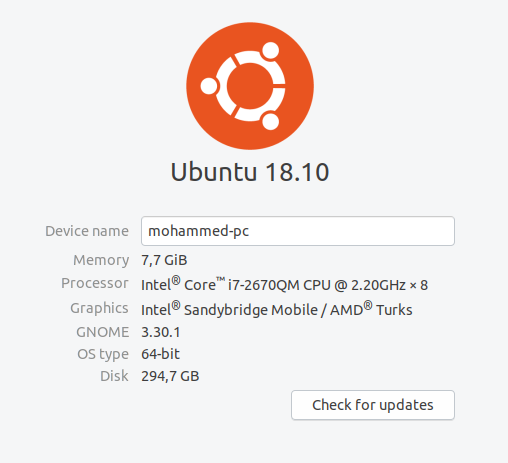
\includegraphics[scale=1.2, frame]{009_os}
\captionsetup{justification=centering}
\caption{The device specification used for testing}
\label{fig:OS}
\end{figure}

The number of sample used for testing is four sample with eleven pathways (bundles) in each side of the brain. The data is collected by \textbf{\textit{UKB Universitätsklinikum Bonn}}. 
\begin{comment}
\begin{center}
\begin{table}[h!]
	\begin{tabular}{| c | c | c | c | c | c | c | c |}
	\hline
	1 & 2 & 3 & 4 & 5 & 6 & 7 & 8\\
	\hline
	(x,y,z) & (x,y,-z) & (x,-y,z) & (x,-y,-z) & (-x,-y,z) & (-x,y,-z) & (-x,y,z) & (-x,-y,-z)\\
	\hline
	\end{tabular}
\caption{$[-1,1]^3$ cube combination}
\label{table:cube}
\end{table}
\end{center}
\end{comment}

The test starts by reading the template and target bundles from \textit{ply} files, then we visualize two graphs and plot the distances between correspondences points in histograms before and after applying PCA. Depend on the result we have and whether PCA improved the alignment or no we decide whether to use PCA or not, if PCA improve the alignment, otherwise we skip it. The figures \{\ref{fig:hist_original}\} \{\ref{fig:img_original}\} \{\ref{fig:hist_PCA}\} \{\ref{fig:img_PCA}\} below show visual orientation and histograms before and after PCA.

\pagebreak

\begin{figure}[h!]
\centering
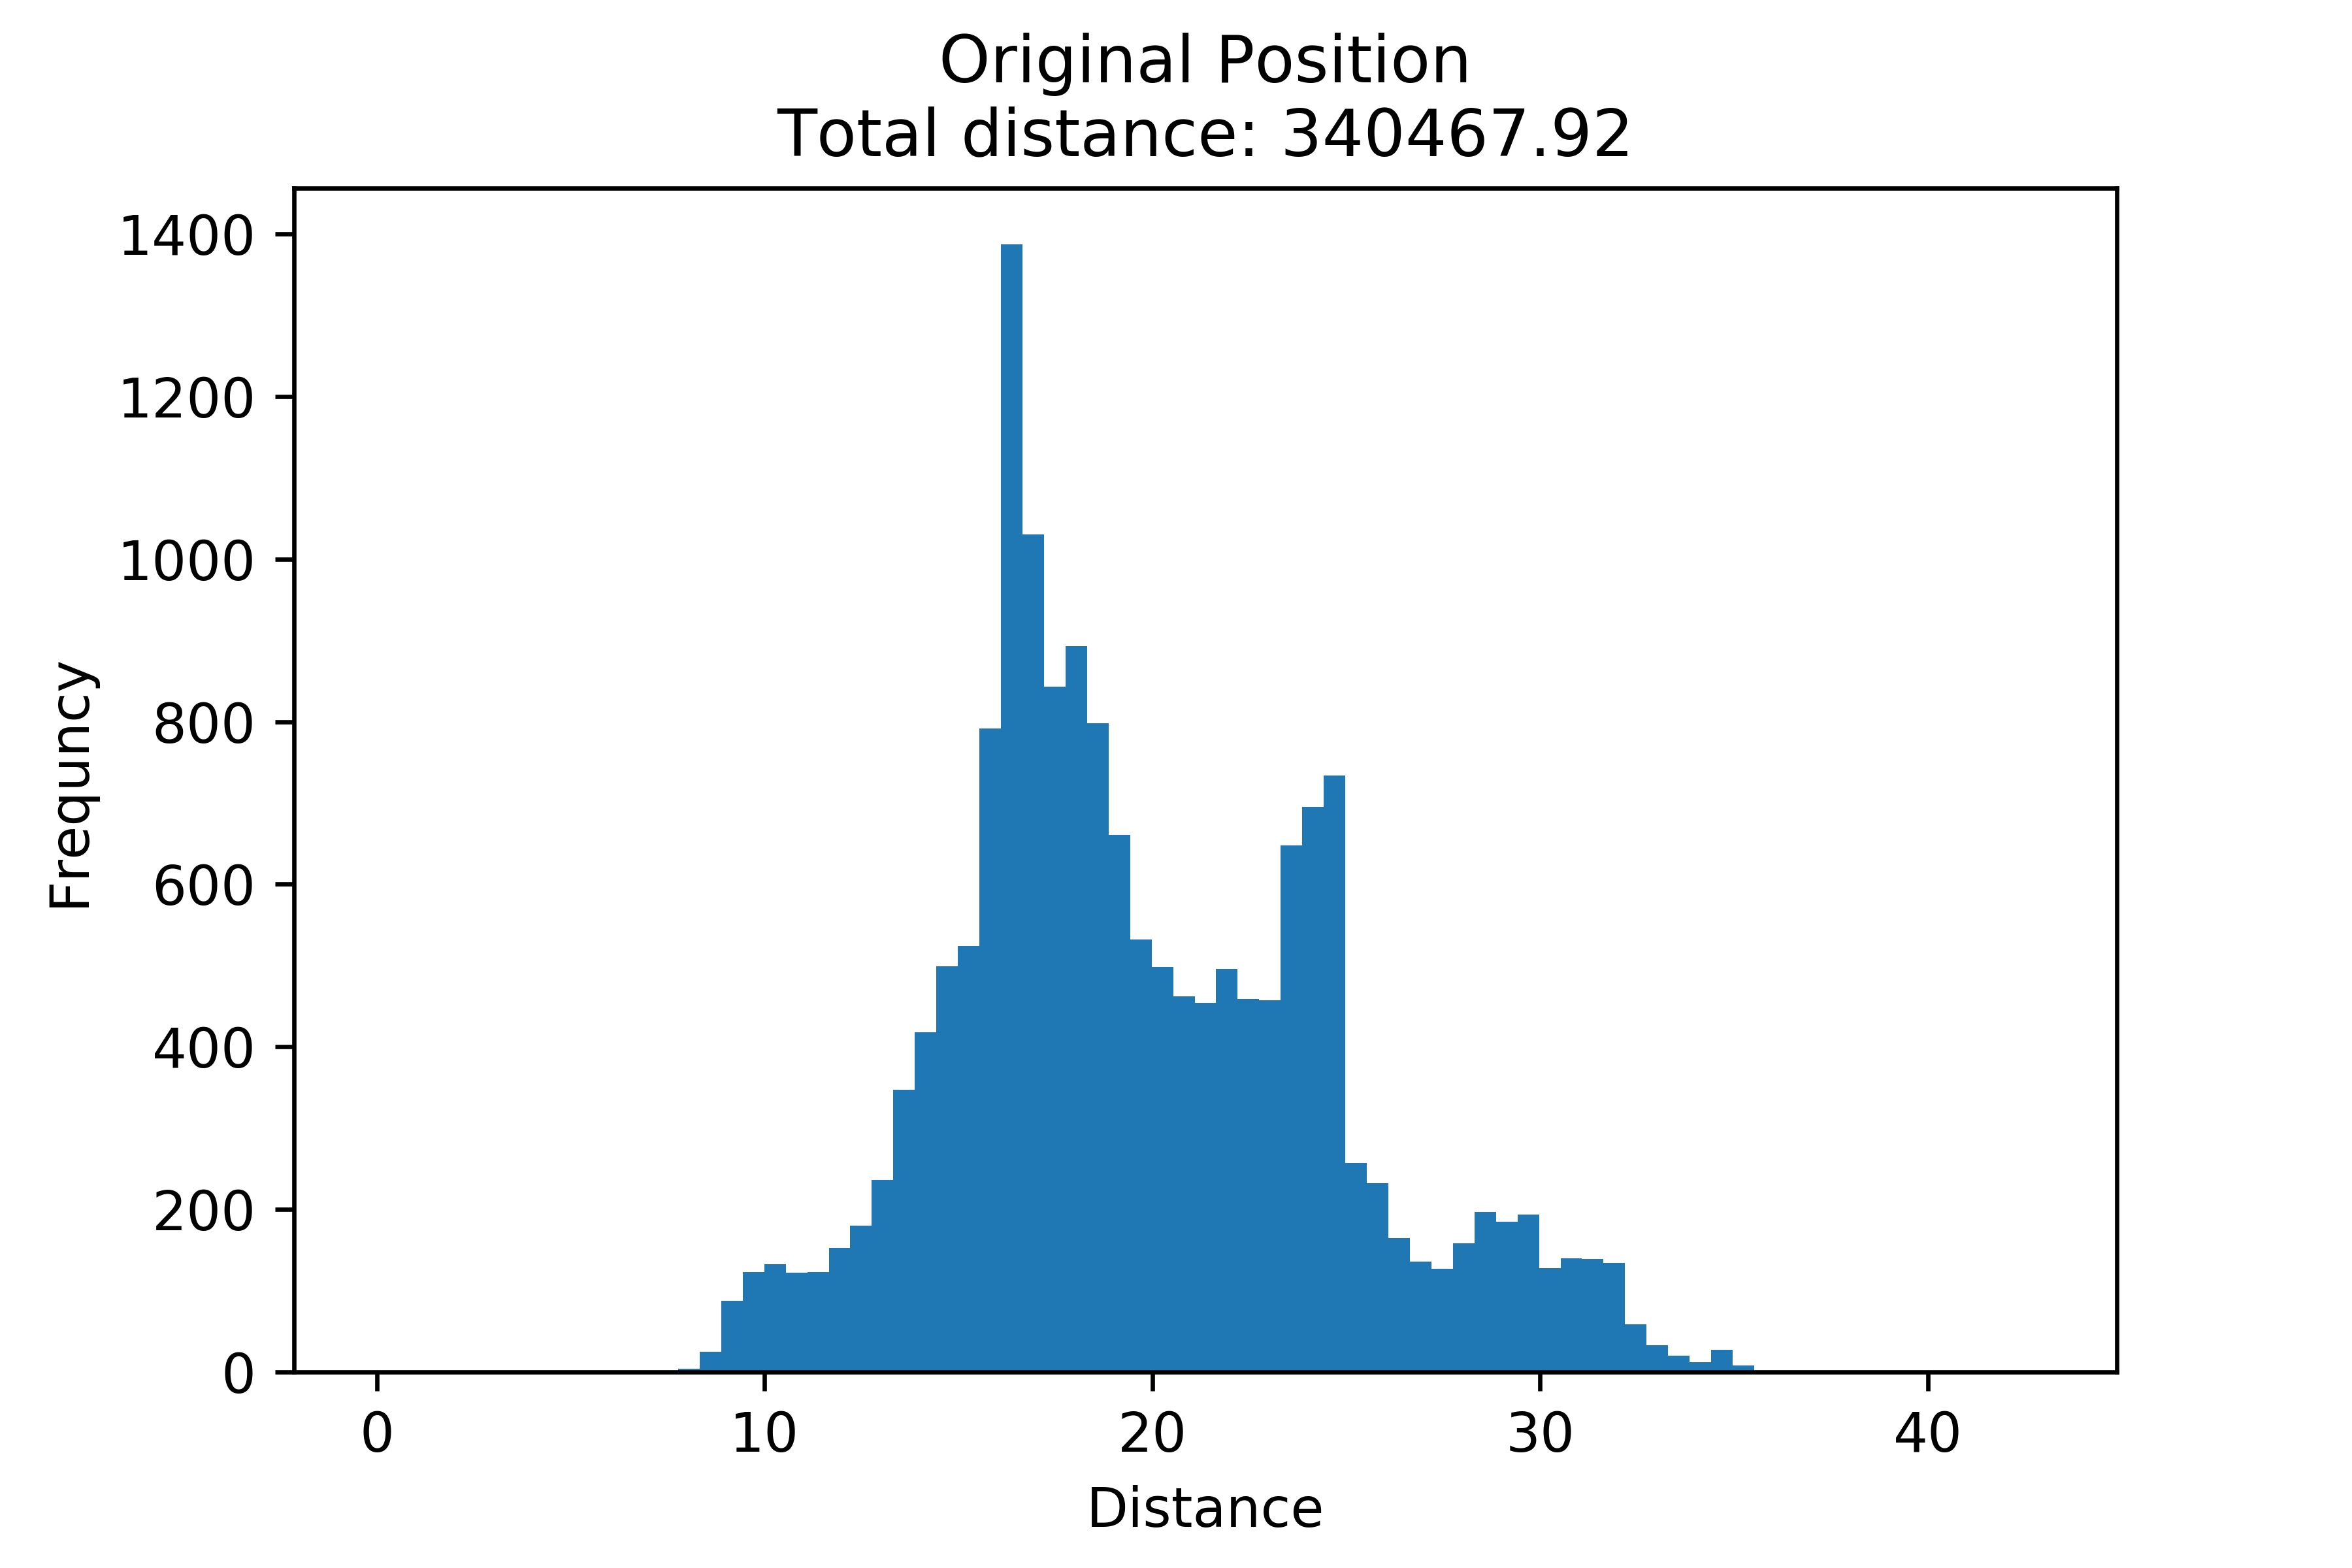
\includegraphics[scale=1]{101_hist_original}
\captionsetup{justification=centering}
\caption{The original distances histogram}
\label{fig:hist_original}
\end{figure}

\begin{figure}[h!]
\centering
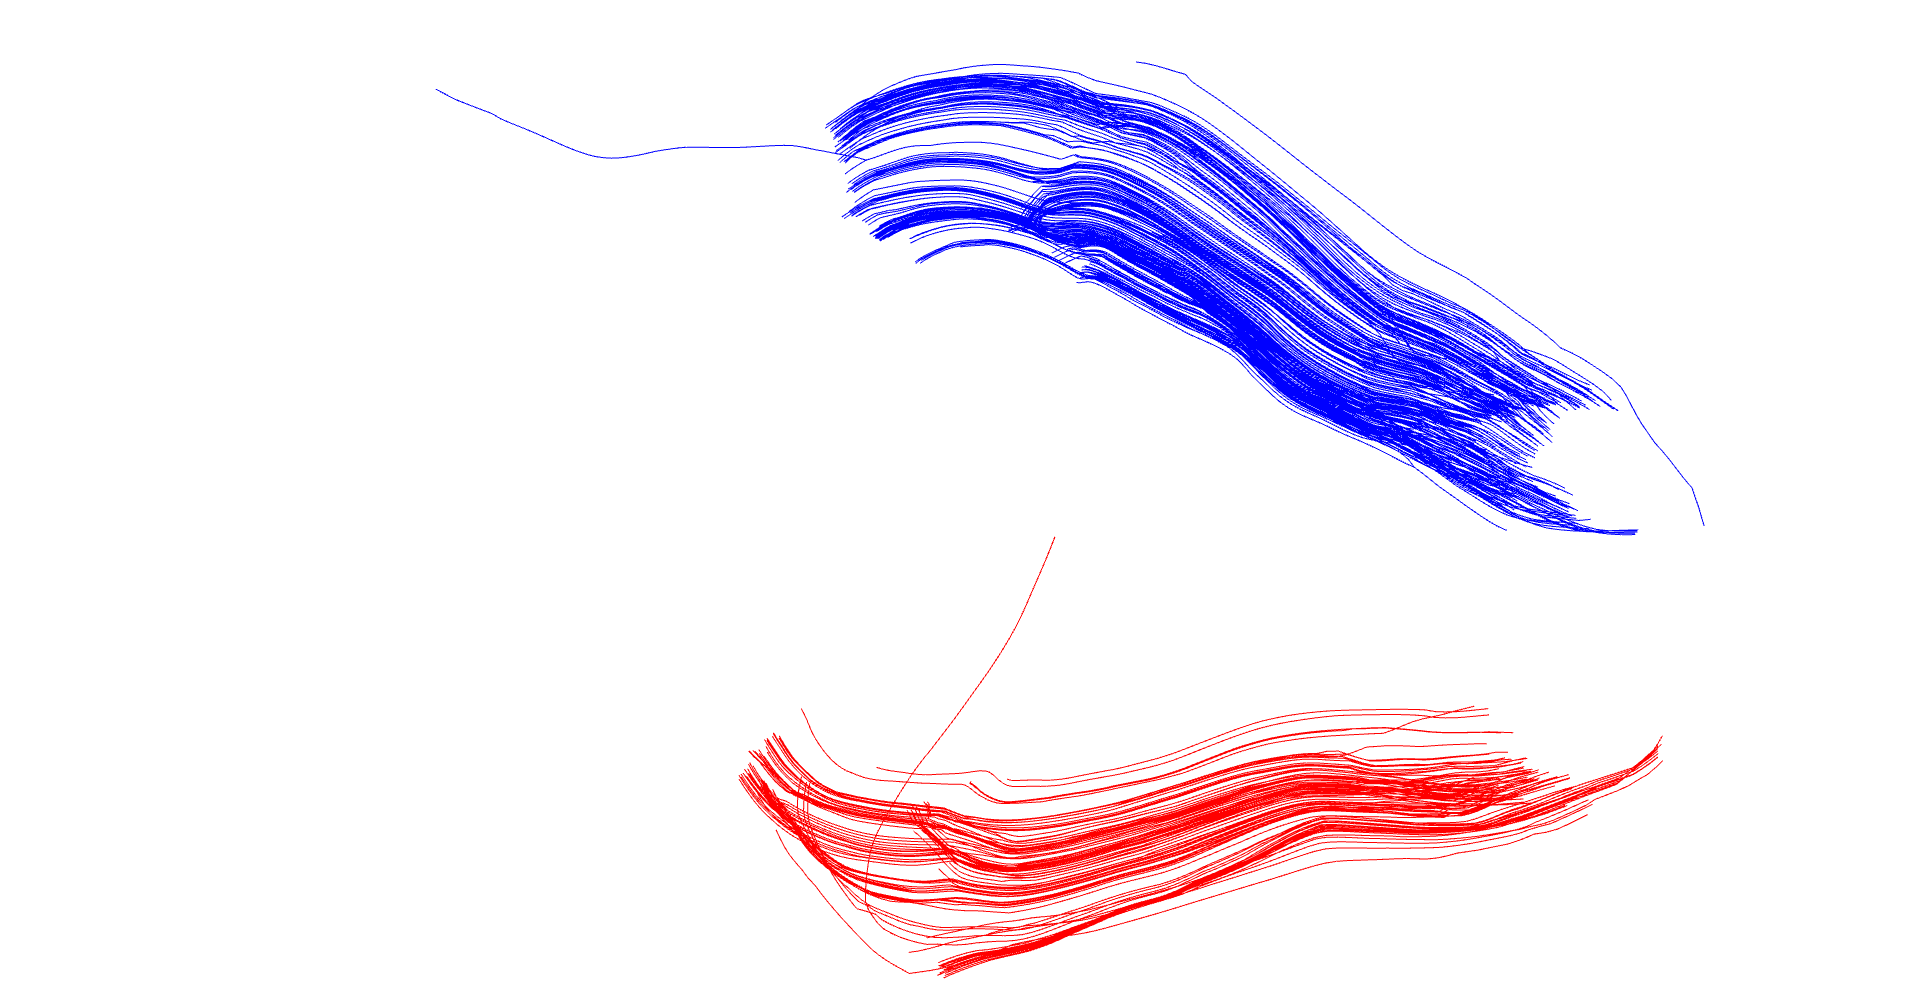
\includegraphics[scale=.8]{101_img_original}
\captionsetup{justification=centering}
\caption{The original orientation}
\label{fig:img_original}
\end{figure}
\pagebreak
\begin{figure}[h!]
\centering
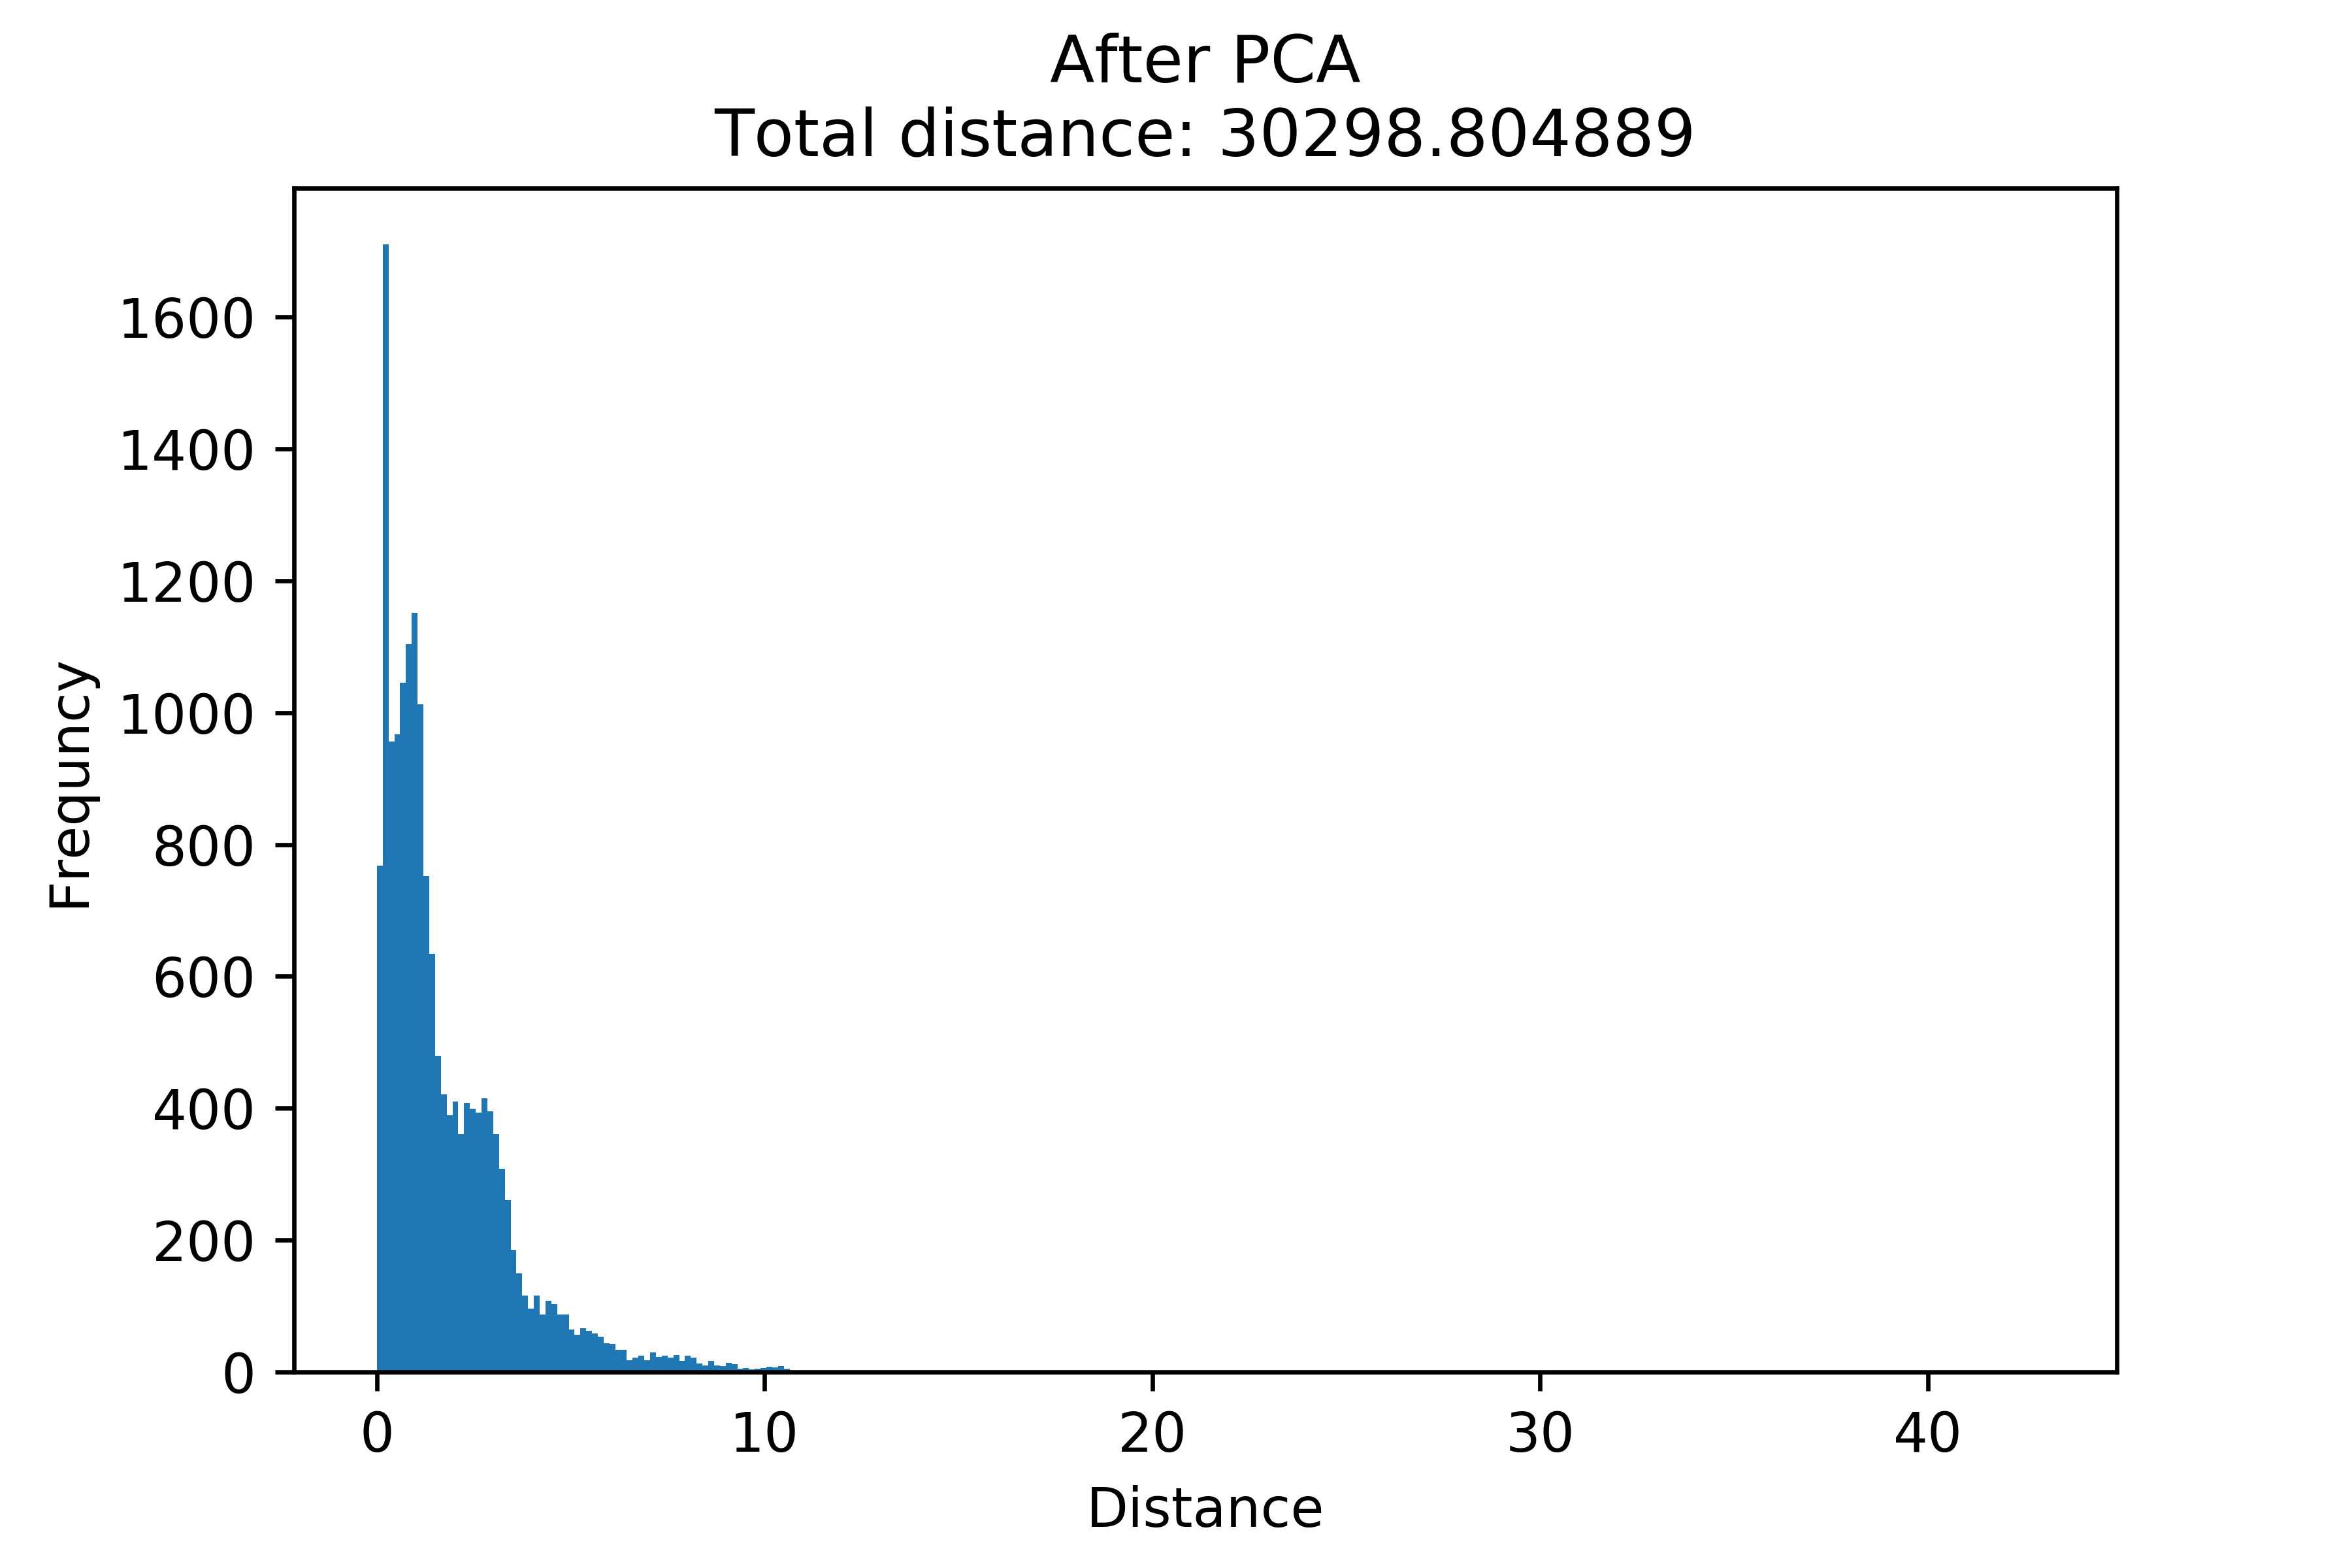
\includegraphics[scale=1]{101_hist_PCA}
\captionsetup{justification=centering}
\caption{The distances histogram after PCA}
\label{fig:hist_PCA}
\end{figure}

\begin{figure}[h!]
\centering
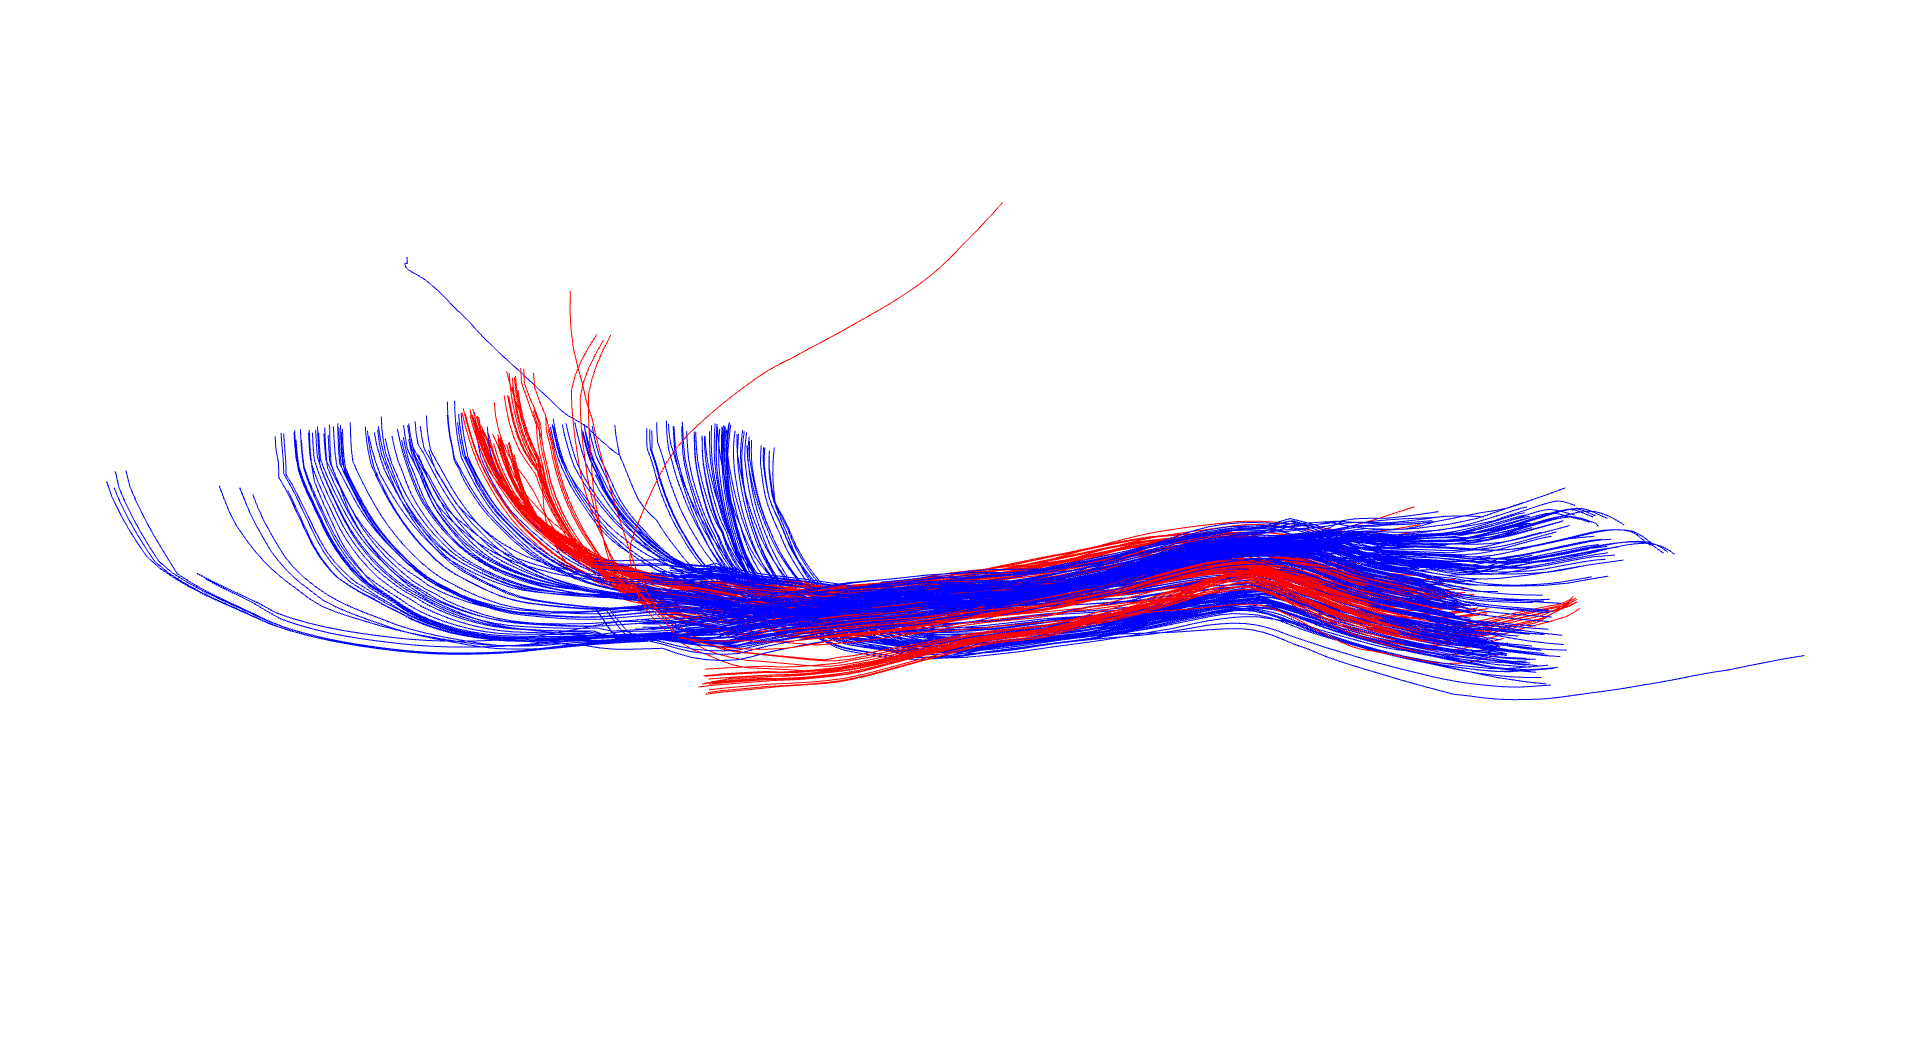
\includegraphics[scale=.3]{101_img_PCA}
\captionsetup{justification=centering}
\caption{The Orientation after PCA}
\label{fig:img_PCA}
\end{figure}
\pagebreak
%\vspace{2em}
When we decide whether to use PCA or not, we run \textit{LSQR} to solve the cost function as illustrated in the previous chapter \textit{Method and Implementation} we get the results in figures \{\ref{fig:hist_ICP}\} \{\ref{fig:img_ICP}\} below, and later we are going to compare them with two other method from \textit{Dipy and non-linear method}

\begin{figure}[h!]
\centering
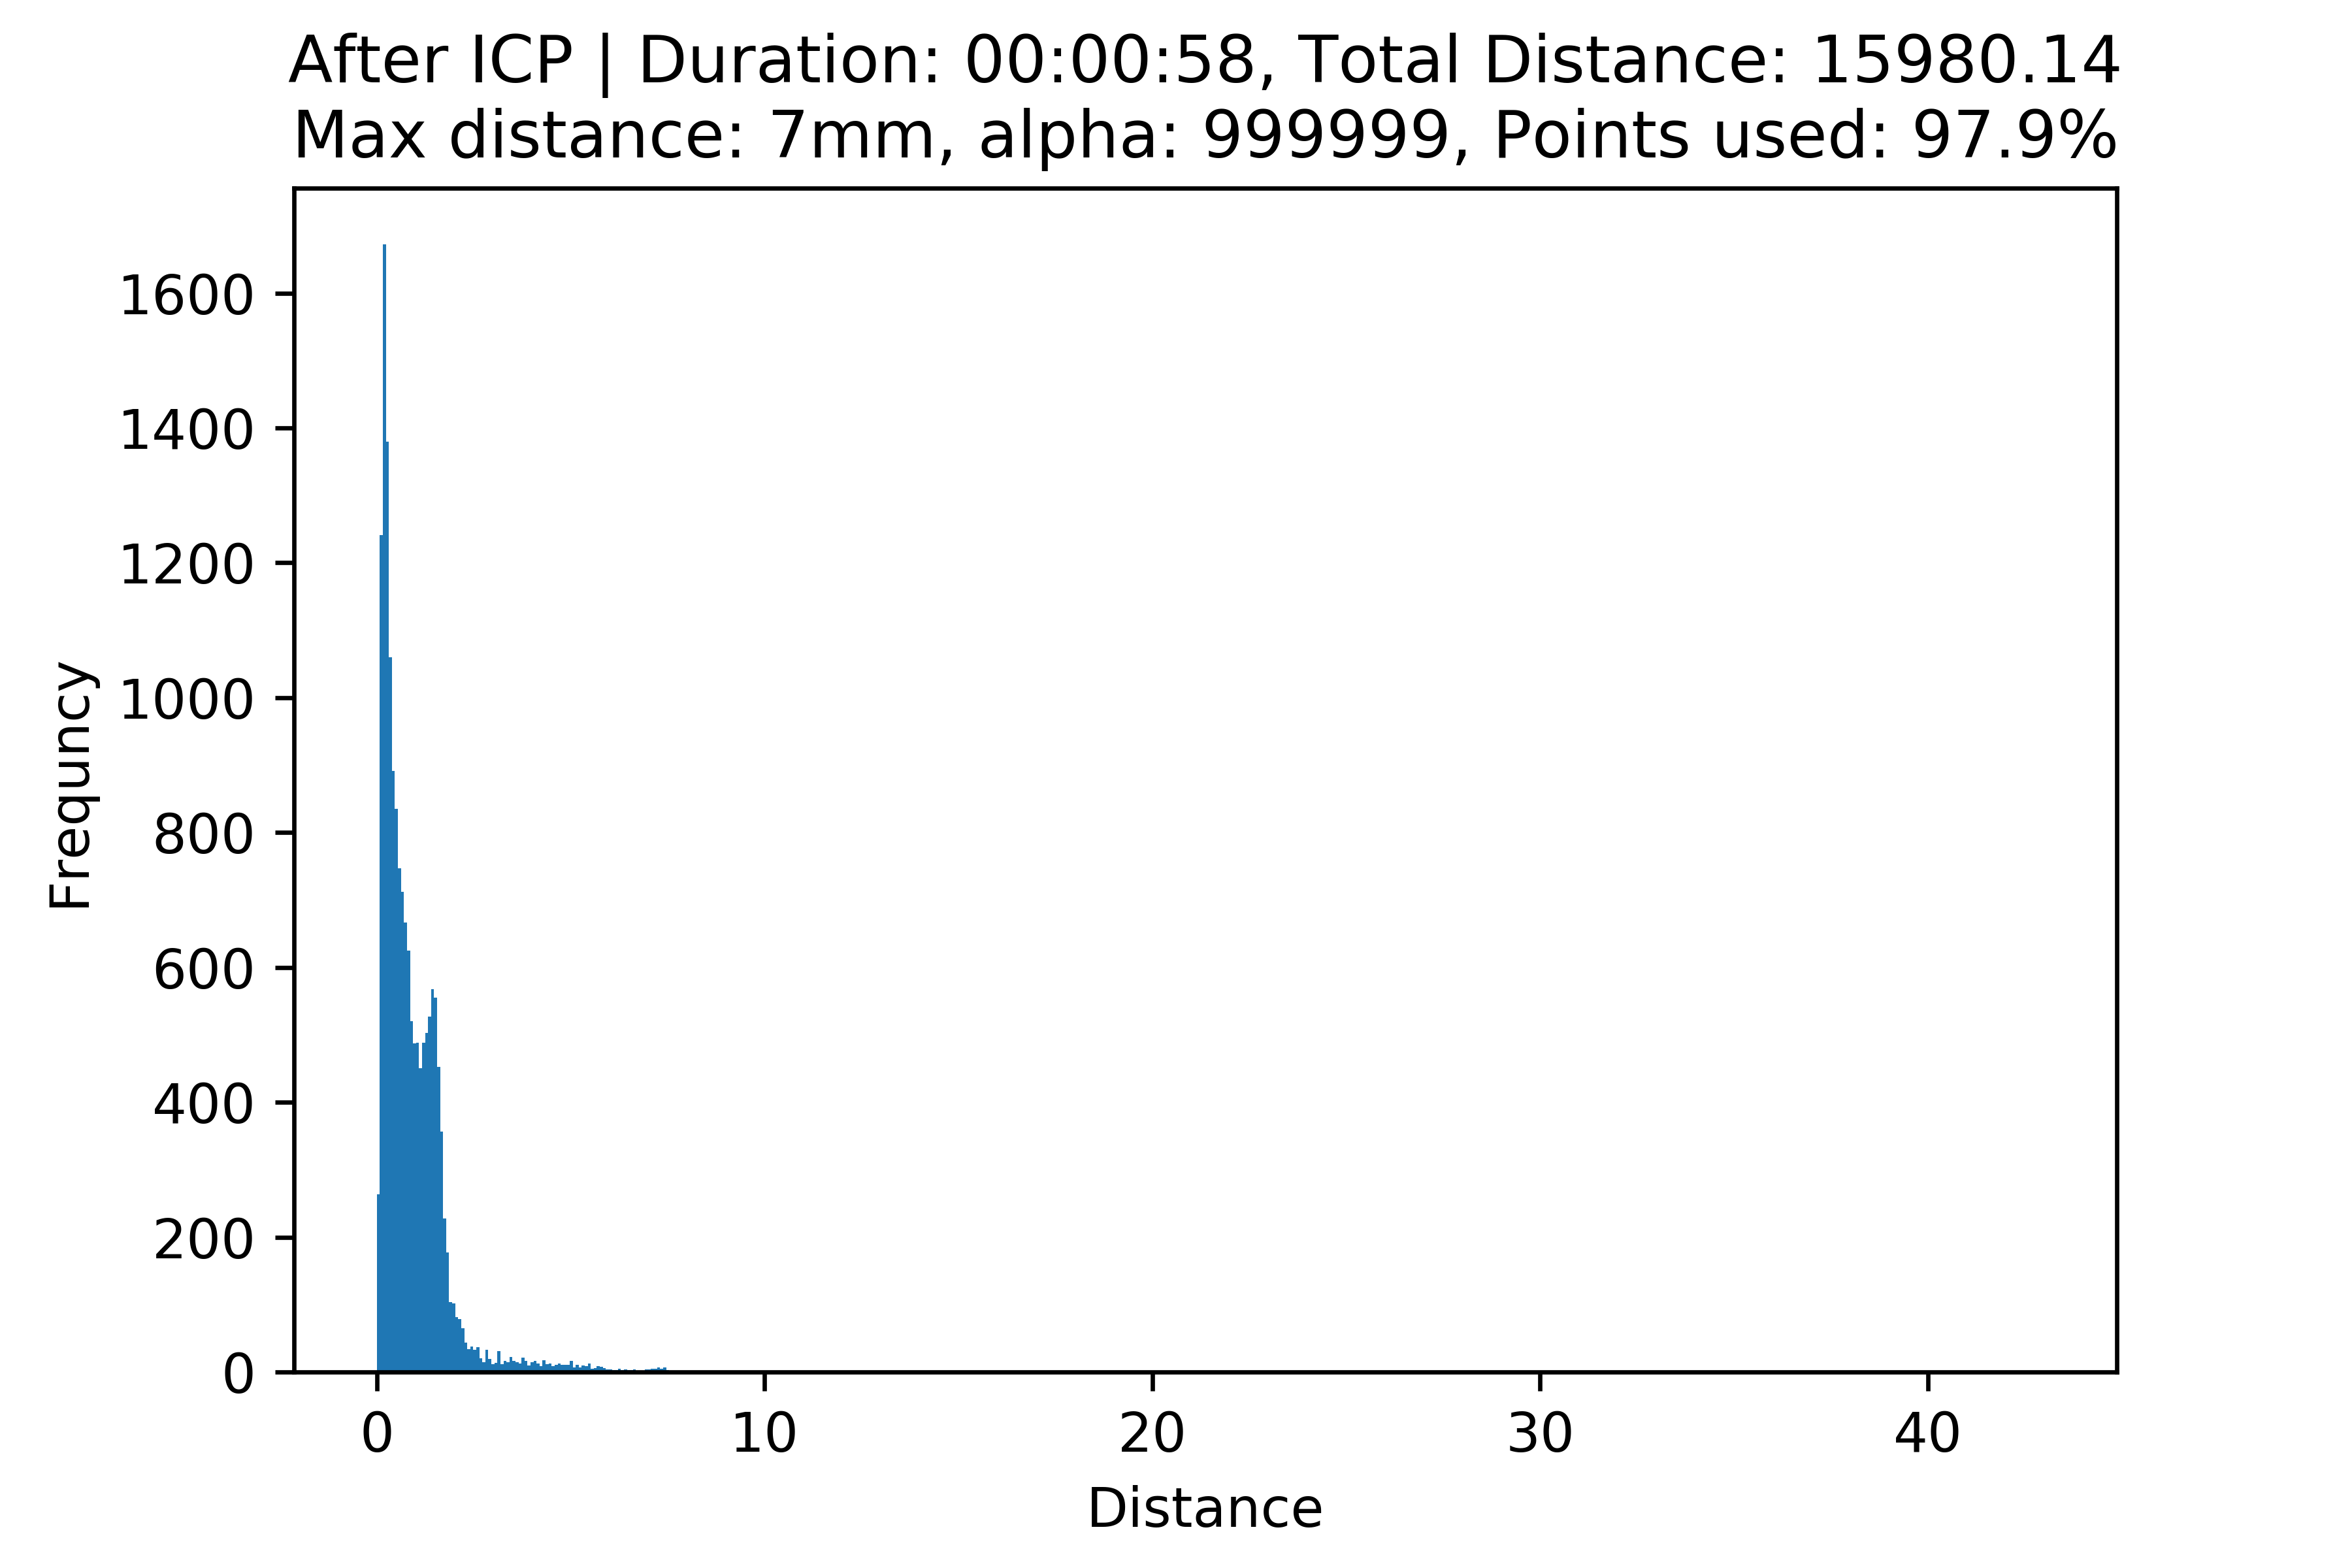
\includegraphics[scale=1]{101_hist_ICP}
\captionsetup{justification=centering}
\caption{The distances histogram after ICP}
\label{fig:hist_ICP}
\end{figure}

\begin{figure}[h!]
\centering
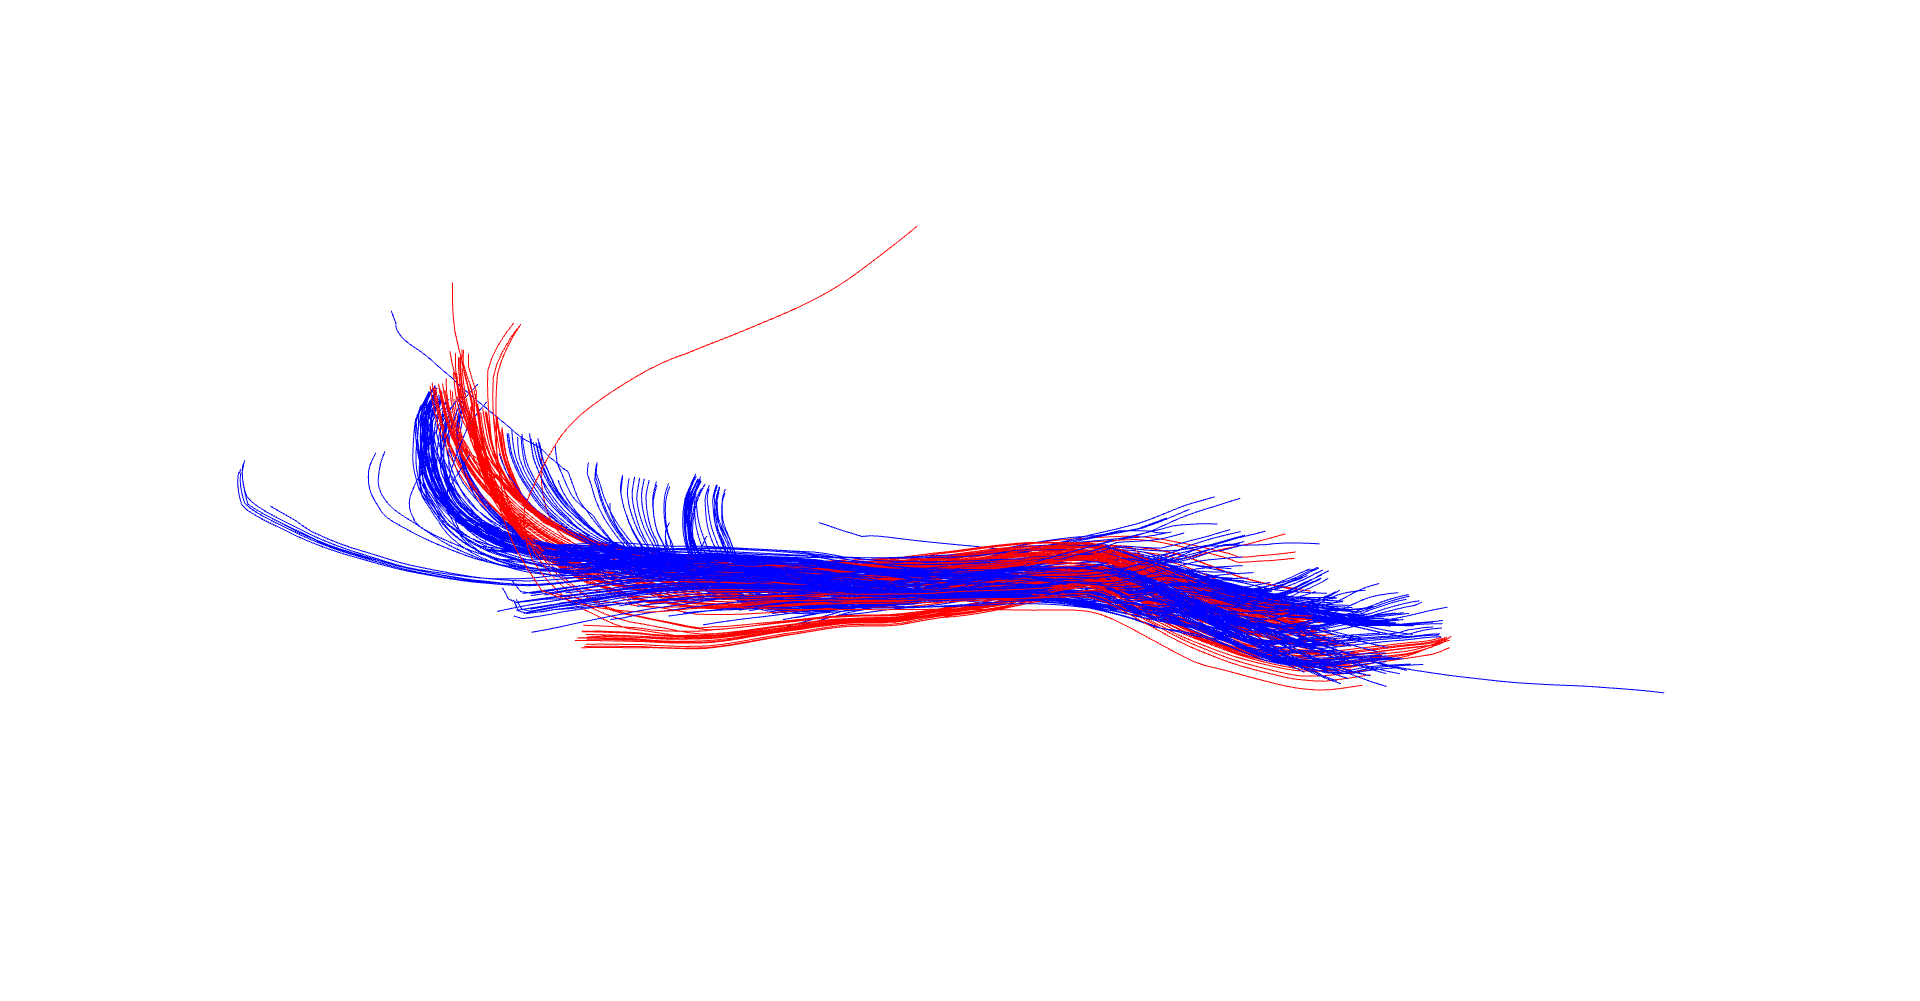
\includegraphics[scale=.4]{101_img_ICP}
\captionsetup{justification=centering}
\caption{The Orientation after ICP}
\label{fig:img_ICP}
\end{figure}
\pagebreak
We align the same bundles with a method discussed in \cite{ODonnell2012} and implemented in \textit{DIPY dipy.align.streamlinear.StreamlineLinearRegistration}. The method get the initial orientation by bringing both graphs to the origin point of the 3D euclidean space, but it does not take care of initial alignment, therefore we used PCA tool that we develop to get the initial alignment and we have the results shown in figures \{\ref{fig:dipy_hist}\} \{\ref{fig:img_dipy}\}

\begin{figure}[h!]
\centering
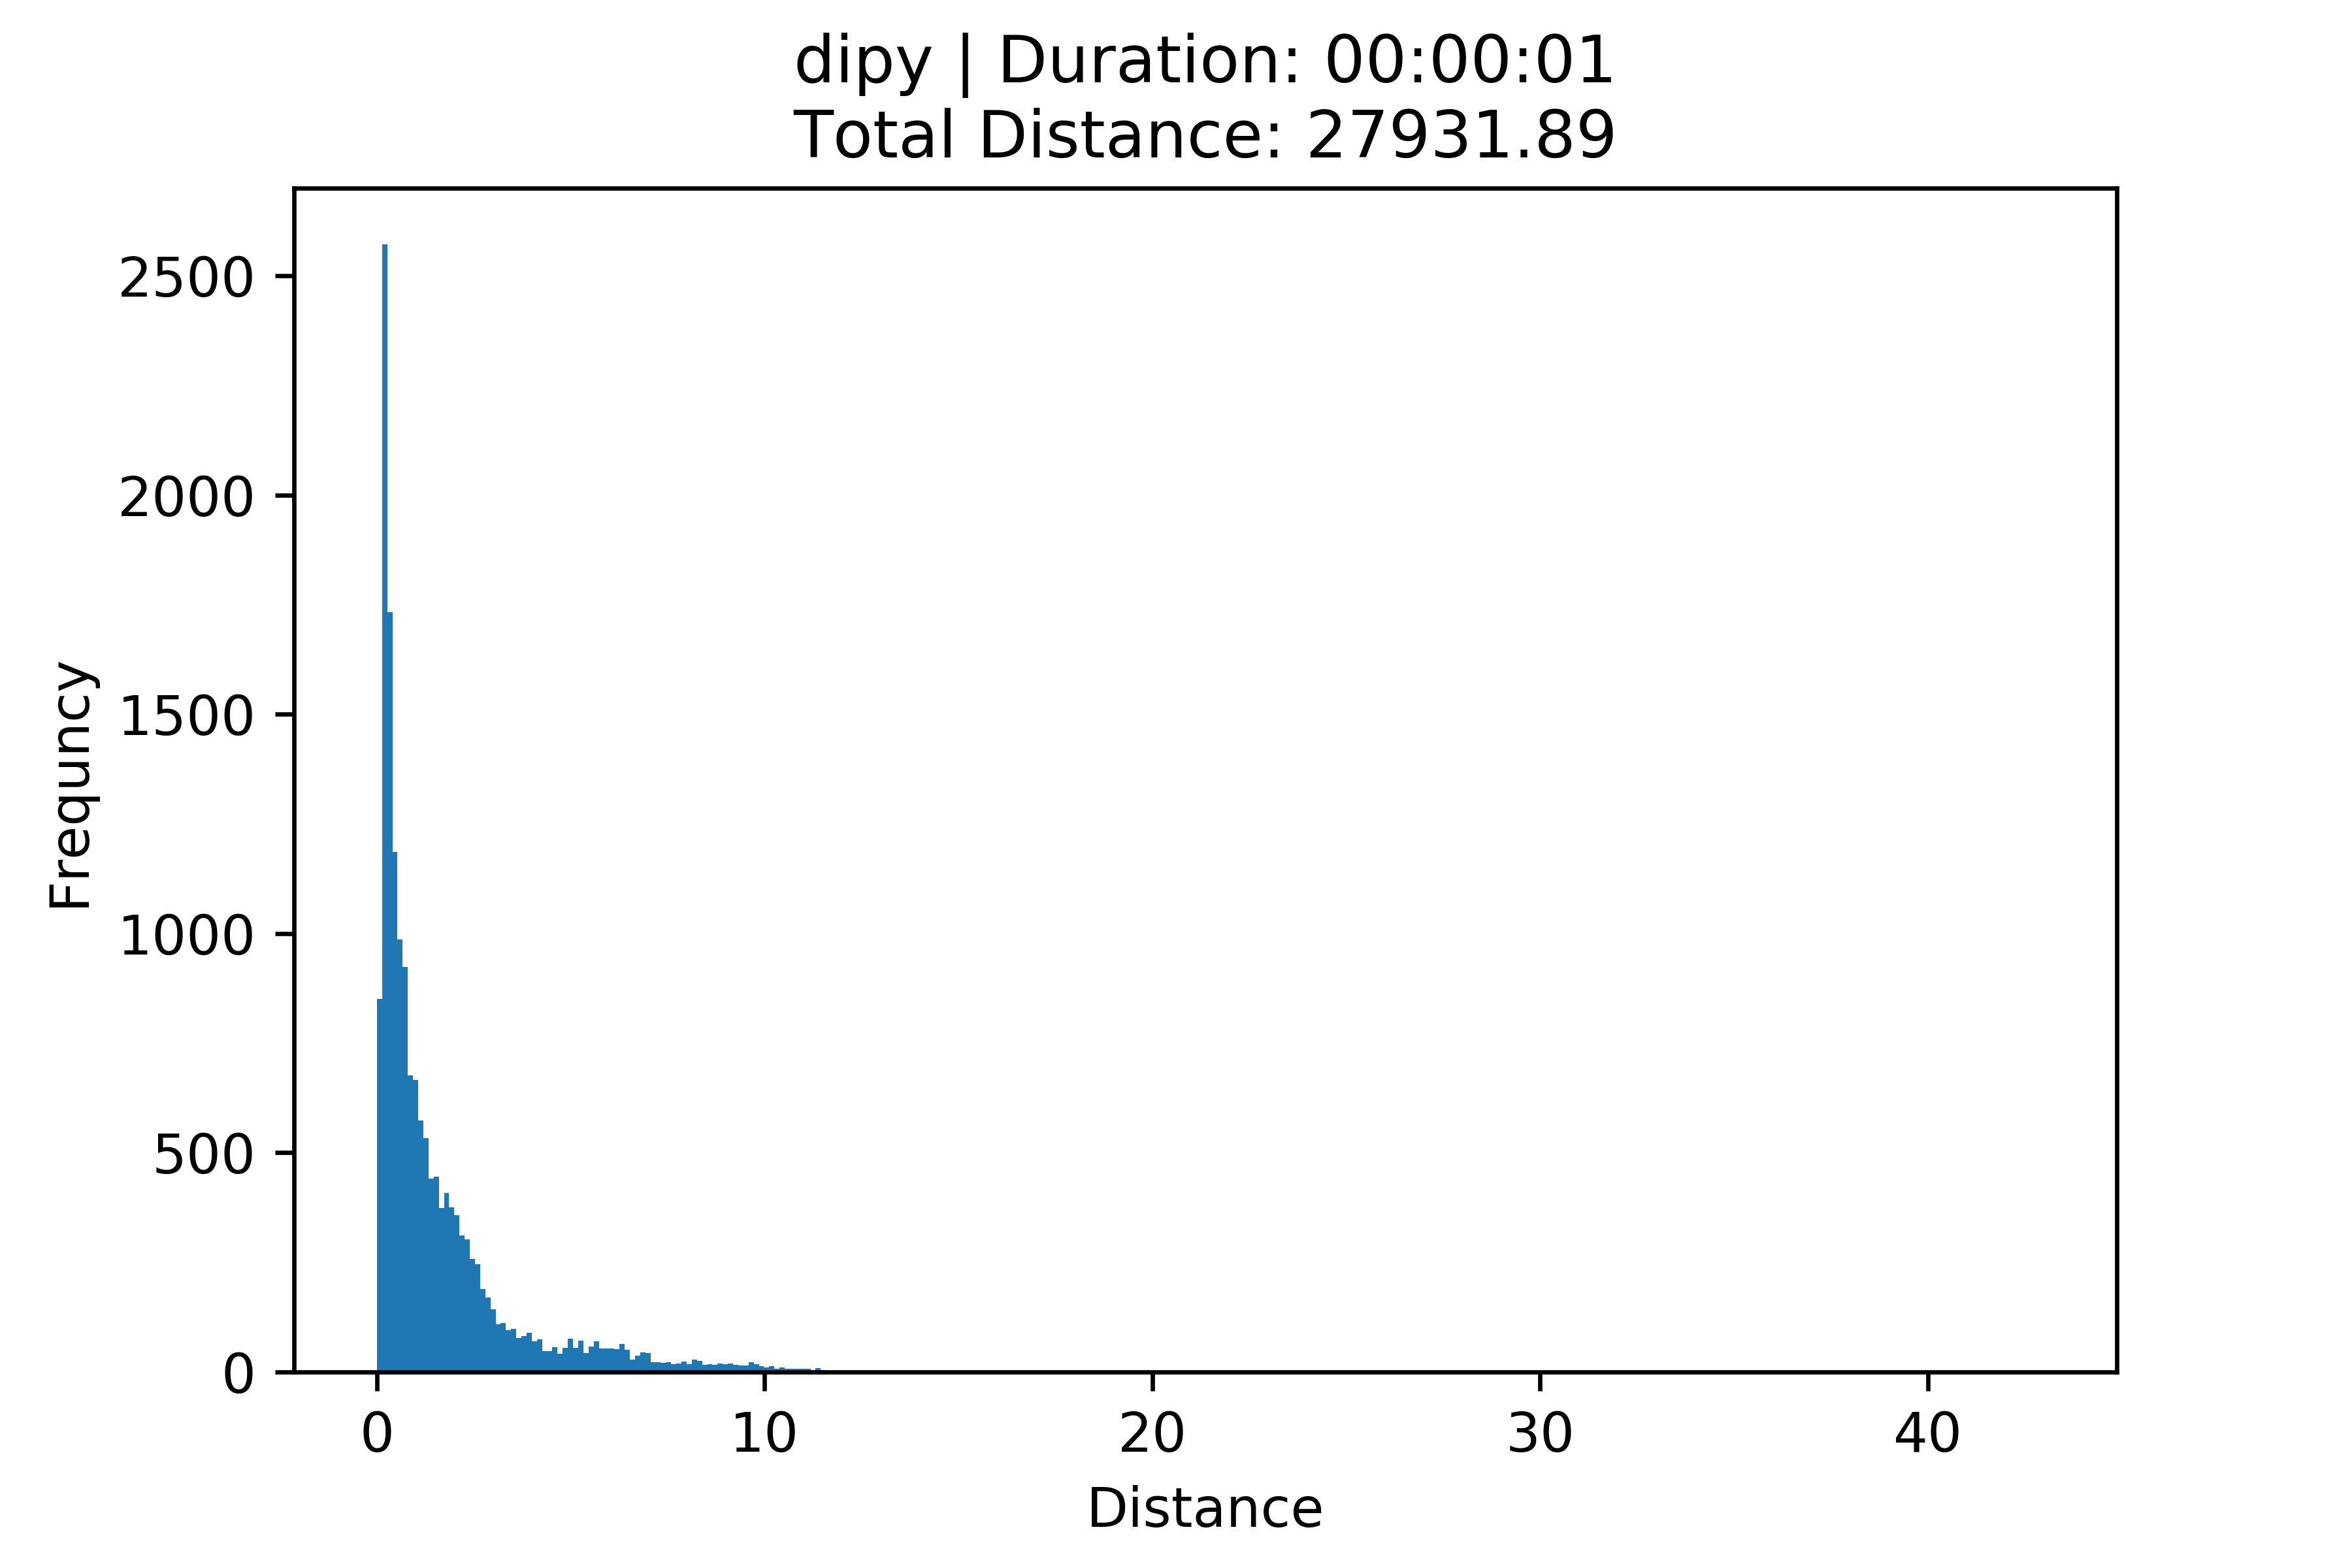
\includegraphics[scale=1]{101_dipy_hist}
\captionsetup{justification=centering}
\caption{The distances histogram after DIPY}
\label{fig:dipy_hist}
\end{figure}

\begin{figure}[h!]
\centering
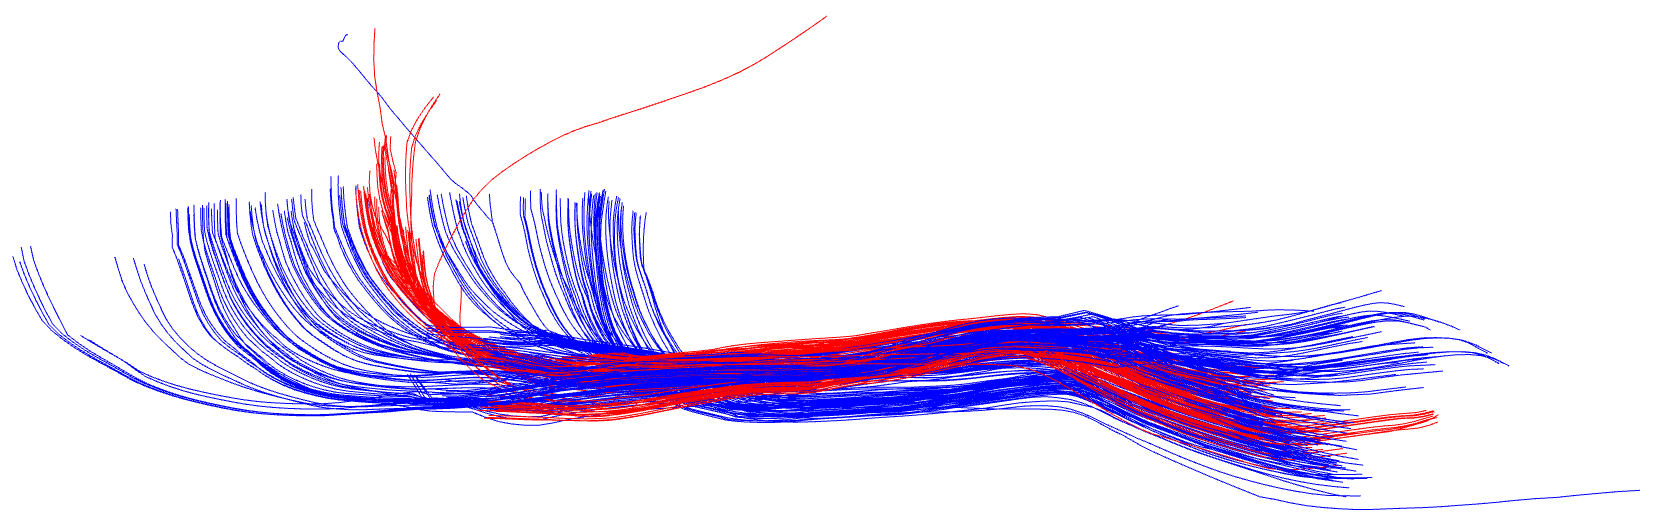
\includegraphics[scale=.3]{101_img_dipy}
\captionsetup{justification=centering}
\caption{The Orientation after DIPY}
\label{fig:img_dipy}
\end{figure}

As it mentioned in \cite{ODonnell2012}, DIPY uses minimum average direct-flip distance (MDF)
\begin{itemize}
\item Time
\item Distance 
\item Visual
\end{itemize}

\end{document}